\chapter{Experimentos}\label{sec:experiments}
%======================================================================================
No presente trabalho, nos concentramos no objetivo proposto descrito na Seção~\ref{sec:objetivos}.

\section{Procedimento}
Primeiramente, filmamos algumas esculturas utilizando a câmera de um \emph{smartphone} convencional na resolução de 1920x1080 pixels. Esta filmagem foi realizada varrendo toda (ou maioria) da superfície da escultura em $360^{\circ}$ com o intuito de ter toda a escultura reconstruída \ref{fig:procedimentoscan}.
Após isso, fizemos mais alguns vídeos, pegando alguns pontos que possuíam mais detalhes e que, com uma única varredura, não era capaz de reproduzir uma boa reconstrução.

\begin{figure}[!h]
	\centering
	%   \includegraphics[width=1.0\linewidth]{figs/3d-curve-sketch/system-diagram.eps}
	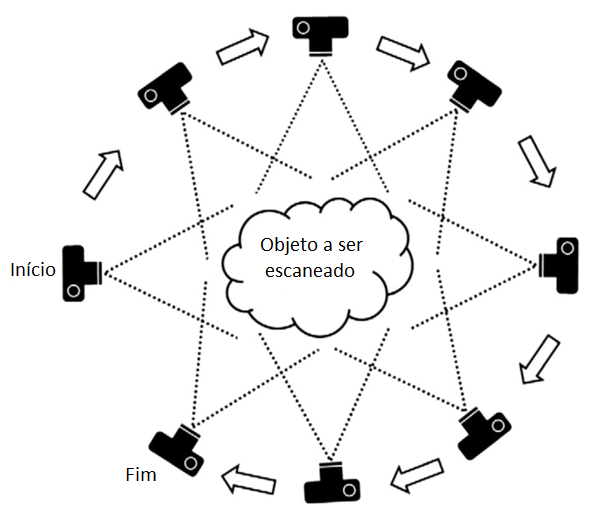
\includegraphics[width=0.4\linewidth]{figs/procedimentoscan.png}
	\caption{%
	Exemplo de como foi realizada a varredura da escultura
	%\cite{Cui:Theobalt:etal:PAMI2013,Pajdla:etal:ICCV2011}.
	}\label{fig:procedimentoscan}
\end{figure}

Com este material, foram feitos "cortes" em determinados \emph{frames} do vídeo, com atenção para não cortar em \emph{frames} muito juntos, pois aumentaria o número de correspondências ambíguas entre as imagens e com isso, o processamento da reconstrução demoraria mais. E não usar \emph{frames} muito distantes, que ocorreria o inverso: com menos correspondências, ficariam buracos (partes sem a informação necessária) na reconstrução, como descrito na Seção \ref{sec:mve}.

Com isso em mente, foram reconstruídas duas esculturas: empregando o VisualSfM, usamos um único vídeo, totalizando 200 imagens. %guerreiro, indio%
Com o MVE, utilizamos dois vídeos, que, ao cortá-los, totalizou cerca de 280 imagens. %sapo%

Além de esculturas ao ar livre, fizemos alguns testes em ambiente fechado, dentro de uma casa, por exemplo. Foi utilizado um objeto feito de cabaça (casca de abóbora) na qual possui uma superfície propícia (Lambertiana)~\cite{basri2003lambertian} para uma reconstrução.

Com o procedimento descrito anteriormente, a partir dos vídeos feitos, obtemos um total de 200 imagens em um vídeo superficial e mais 24 imagens mais detalhadas do objeto, ambos numa resolução de 1080x1920 pixels. E, para um mesmo conjunto de imagens, rodamos tanto o VisualSfM quanto o MVE.

\subsection{Resultados da reconstrução do objeto com o VisualSfM}

Seguindo o passo-a-passo de reconstrução do software, obtivemos os seguintes resultados:

%COLOCAR IMAGENS GUERREIRO AQUI%


%-------------------GALINHA A PARTIR DAQUI----------------------------------%

Para o ambiente fechado, conseguimos os resultados, apenas com o primeiro vídeo, de 200 imagens:

\begin{table}[h!]
\caption{Tempos obtidos da reconstrução do objeto usando o VisualSfM}
\label{tab:temposSfM}
\begin{tabular}{|l|p{4.7cm}|}
\hline
Procedimento & Tempo (aprox.) \\ \hline
Carregamento de imagens & 50 segundos \\ \hline
Calcular pares correspondentes de \emph{features} & 159 segundos \\ \hline
Gerar a reconstrução esparsa do modelo & 135 segundos \\ \hline
Gerar a reconstrução densa do modelo & 1.416 segundos \\ \hline
\end{tabular}
\end{table}

A figura \ref{fig:reconstrucaoEsparsaVisualSFM} mostra o resultado da reconstrução esparsa do algoritmo PBA. Não é tão nítida como na reconstrução densa ~\ref{fig:reconstrucaoDensaVisualSFM}, a quantidade de ruídos, provenientes de outros objetos presentes na cena (o VisualSfM só identifica objetos estáticos). Só é possível limpar a malha manualmente, pressionando a tecla F1 e selecionando a área desejada para ser deletada. Não é muito prático, pois podemos excluir alguns pontos importantes, o ideal seria fazer esta limpeza por meio de programas externos.

\begin{figure}[!h]
	\centering
	%   \includegraphics[width=1.0\linewidth]{figs/3d-curve-sketch/system-diagram.eps}
	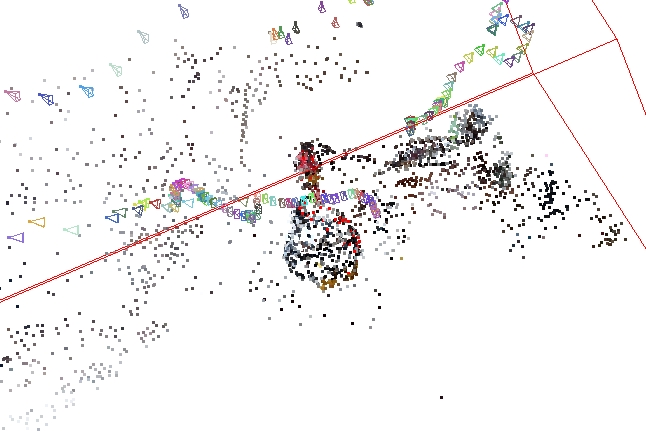
\includegraphics[width=0.3\linewidth]{figs/galinhasparsa.jpg}
	\caption{%
	Reconstrução esparsa do objeto no VisualSfM com 200 imagens.
	%\cite{Cui:Theobalt:etal:PAMI2013,Pajdla:etal:ICCV2011}.
	}\label{fig:reconstrucaoEsparsaVisualSFM}
\end{figure}

\begin{figure}[!h]
	\centering
	%   \includegraphics[width=1.0\linewidth]{figs/3d-curve-sketch/system-diagram.eps}
	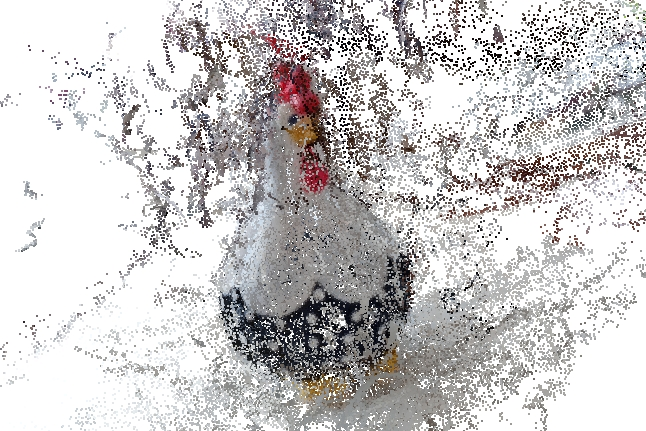
\includegraphics[width=0.3\linewidth]{figs/galinhadense.jpg}
	\caption{%
	Reconstrução densa do objeto no VisualSfM com 200 imagens.
	%\cite{Cui:Theobalt:etal:PAMI2013,Pajdla:etal:ICCV2011}.
	}\label{fig:reconstrucaoDensaVisualSFM}
\end{figure}

Fizemos uma outra reconstrução, utilizando os dois vídeos (gerando 224 imagens). Caso usássemos um conjunto maior, o programa parava de funcionar por falta de memória, mesmo após ajustar parâmetros (como o número de vizinhos, número de \emph{cores} do processador, \emph{level} do PMVS, entre outros) para melhorar esse problema. Portanto, o experimento seguiu da forma:

\begin{table}[h!]
\caption{Tempos obtidos da reconstrução do objeto, com 224 imagens usando o VisualSfM}
\label{tab:temposSfM224}
\begin{tabular}{|l|p{4.7cm}|}
\hline
Procedimento & Tempo (aprox.) \\ \hline
Carregamento de imagens & 60 segundos \\ \hline
Calcular pares correspondentes de \emph{features} & 200 segundos \\ \hline
Gerar a reconstrução esparsa do modelo & 162 segundos \\ \hline
Gerar a reconstrução densa do modelo & 1920 segundos \\ \hline
\end{tabular}
\end{table}

Percebemos que não foi tão proveitoso (qualitativamente) usar mais imagens neste caso, inclusive o algoritmo perdeu a referência do objeto e gerou um segundo modelo na reconstrução esparsa \ref{fig:reconstrucaoEsparsaVisualSFM224}, e consequentemente, na reconstrução densa \ref{fig:reconstrucaoDensaVisualSFM2241} e \ref{fig:reconstrucaoDensaVisualSFM2242}. O que gerou uma cerca incoerência na reconstrução.

\begin{figure}[!h]
	\centering
	%   \includegraphics[width=1.0\linewidth]{figs/3d-curve-sketch/system-diagram.eps}
	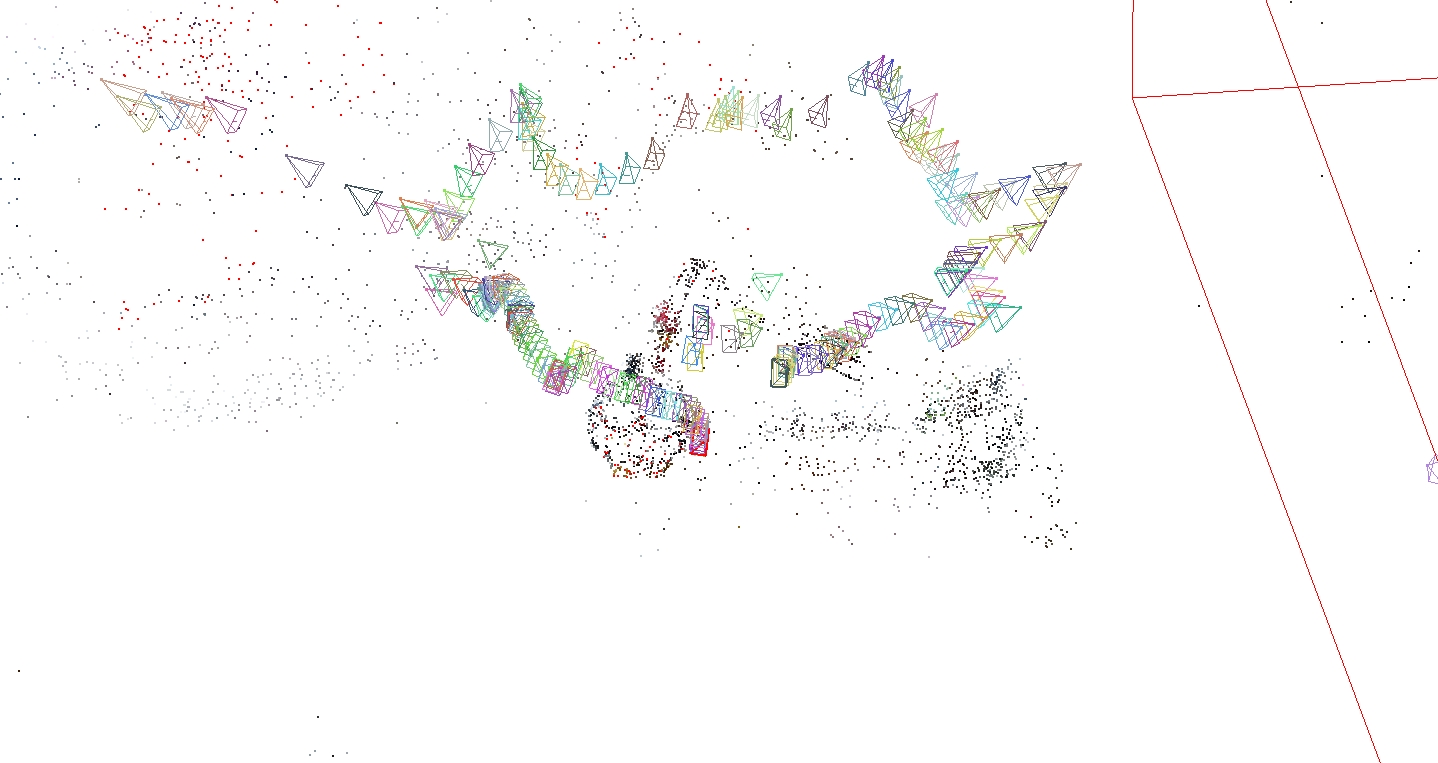
\includegraphics[width=0.5\linewidth]{figs/perto_longe_esparsa.jpg}
	\caption{%
	Reconstrução esparsa do objeto com 224 imagens no VisualSfM.
	%\cite{Cui:Theobalt:etal:PAMI2013,Pajdla:etal:ICCV2011}.
	}\label{fig:reconstrucaoEsparsaVisualSFM224}
\end{figure}

\begin{figure}[!h]
	\centering
	%   \includegraphics[width=1.0\linewidth]{figs/3d-curve-sketch/system-diagram.eps}
	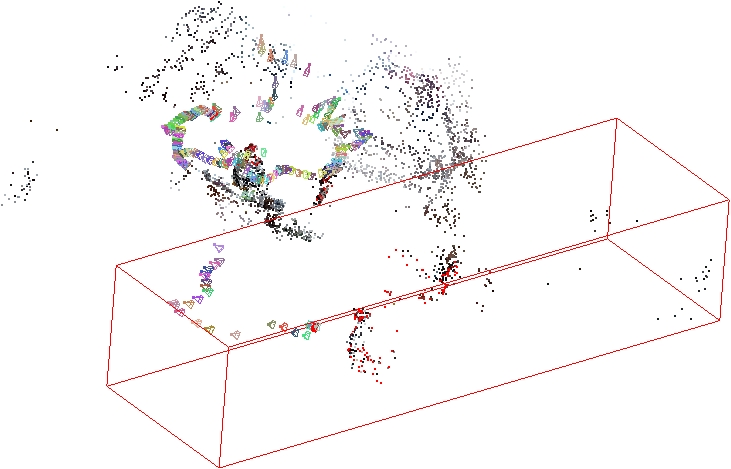
\includegraphics[width=0.5\linewidth]{figs/perto_longe_esparsa_2.jpg}
	\caption{%
	Foram gerados dois modelos esparsos do objeto a partir do conjunto inicial de 224 imagens, provavelmente, proveniente da falta de parâmetros da câmera.
	%\cite{Cui:Theobalt:etal:PAMI2013,Pajdla:etal:ICCV2011}.
	}\label{fig:reconstrucaoEsparsaVisualSFM224}
\end{figure}

\begin{figure}[!h]
	\centering
	\subfloat[(a)]{\label{fig:reconstrucaoDensaVisualSFM2241}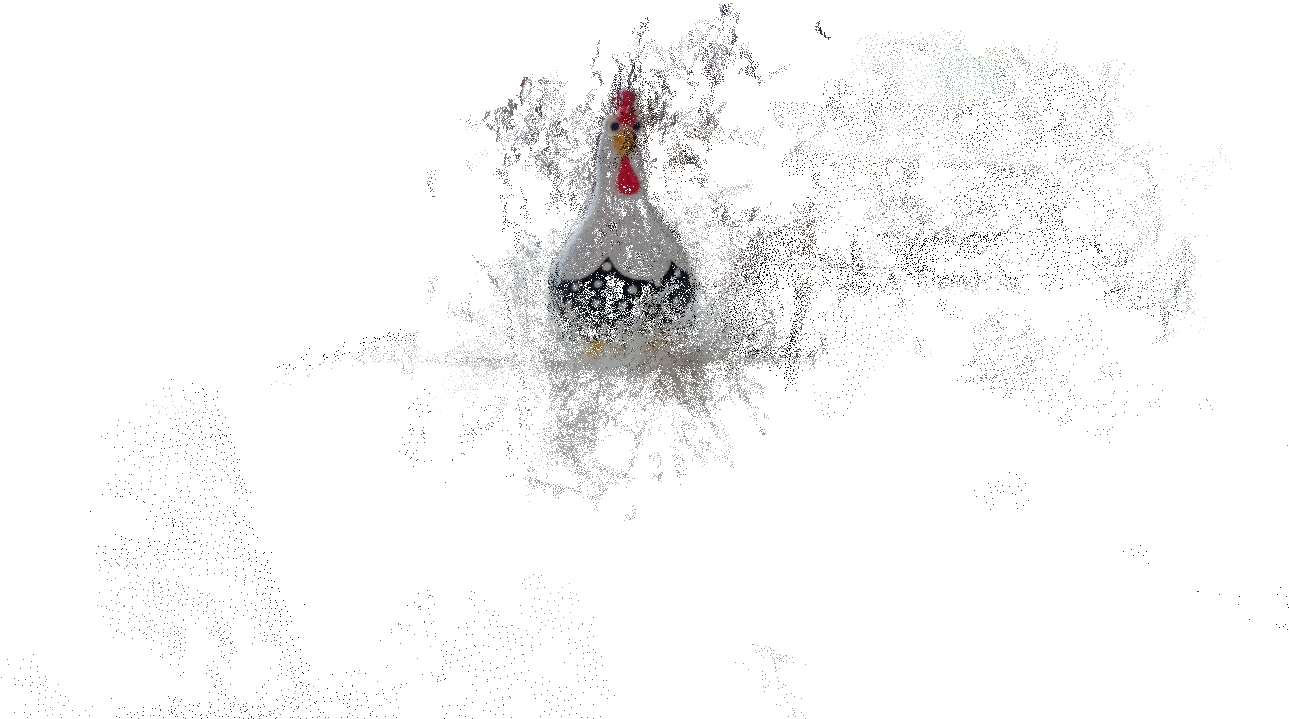
\includegraphics[width=0.5\linewidth]{figs/galinhadense224.jpg}}
	\subfloat[(b)]{\label{fig:reconstrucaoDensaVisualSFM2242}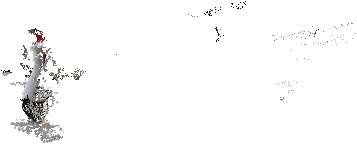
\includegraphics[width=0.5\linewidth]{figs/galinhavisualsfm224.jpg}}
	\caption{Reconstruções densas do primeiro (a) e do segundo (b) modelo do objeto no VisualSfM com 224 imagens.
	}
\end{figure}

%------------------ACABOU SFM---------------------------------------------%

\subsection{Resultados da reconstrução do objeto com o MVE}

A utilização do software é bem intuitiva, seja por linha de comando ou pela interface gráfica (neste modo, fica mais fácil visualizar cada etapa da reconstrução). Amplamente configurável, podendo escolher a vizinhança, escala, manter o mapa de profundidade, ver os dados \emph{EXIF} de cada imagem, dentre outras configurações.

Entretanto, para a aplicação proposta neste projeto, não é muito interessante, visto que ele utiliza a informação das câmeras, inseridas nas imagens (\emph{EXIF}) e como as imagens empregadas na reconstrução são, tecnicamente, vídeos cortados em determinados \emph{frames}, não é possível obter a informação das câmeras~\ref{fig:mveexif}. Logo o software não tem tanta aplicabilidade neste caso, pois recai no problema dos parâmetros padrões adotados para as câmeras não serem bons o suficiente para estes conjuntos de dados, a menos que sejam tiradas fotos sequenciais de alguma escultura ou objeto que se deseja gerar a reconstrução densa, pois dessa forma, as informações necessárias das câmeras estarão armazenadas.

\begin{figure}[!h]
	\centering
	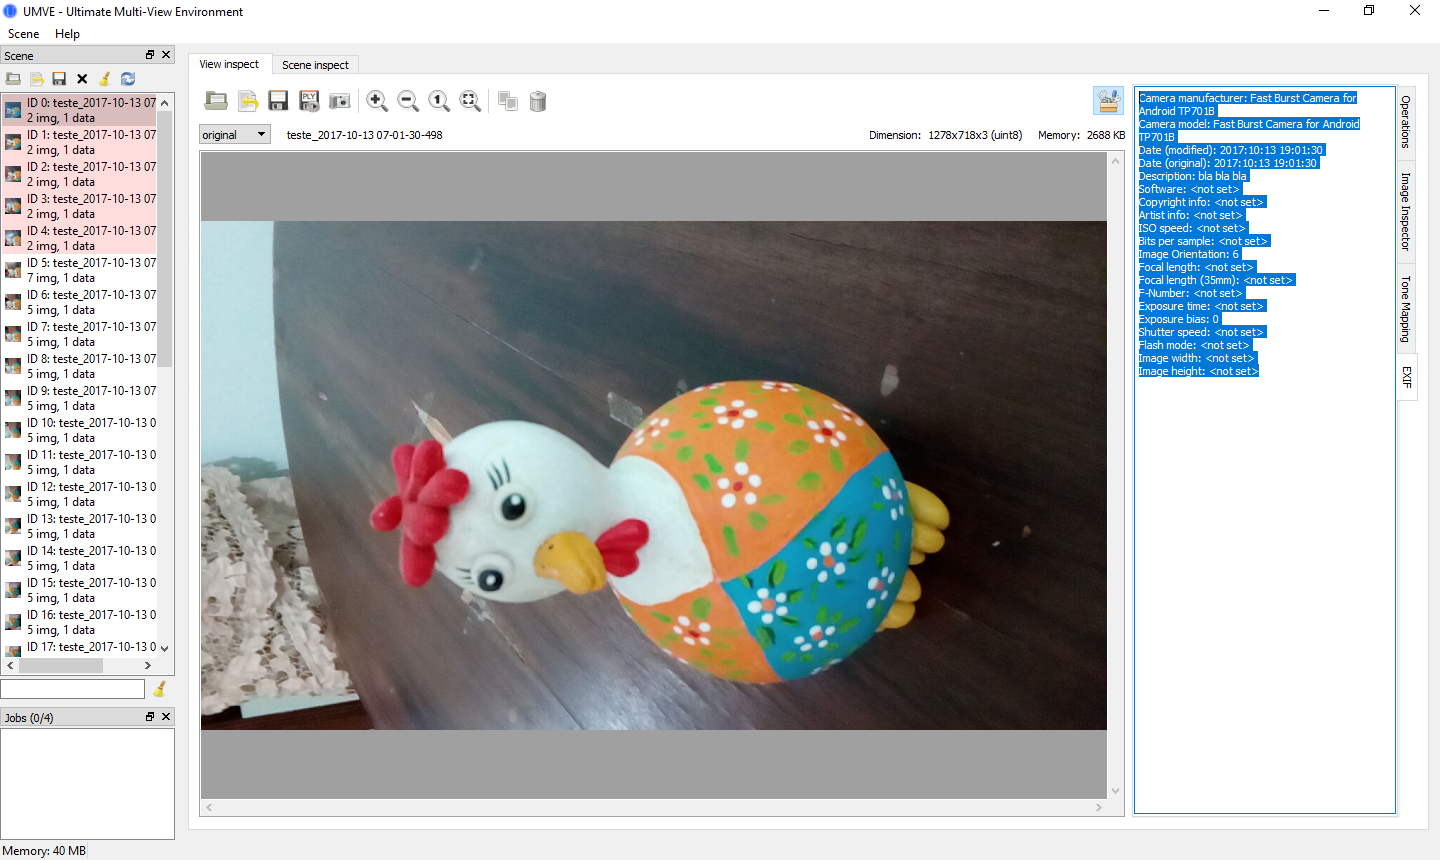
\includegraphics[width=0.5\linewidth]{figs/exifumve.png}(a)
	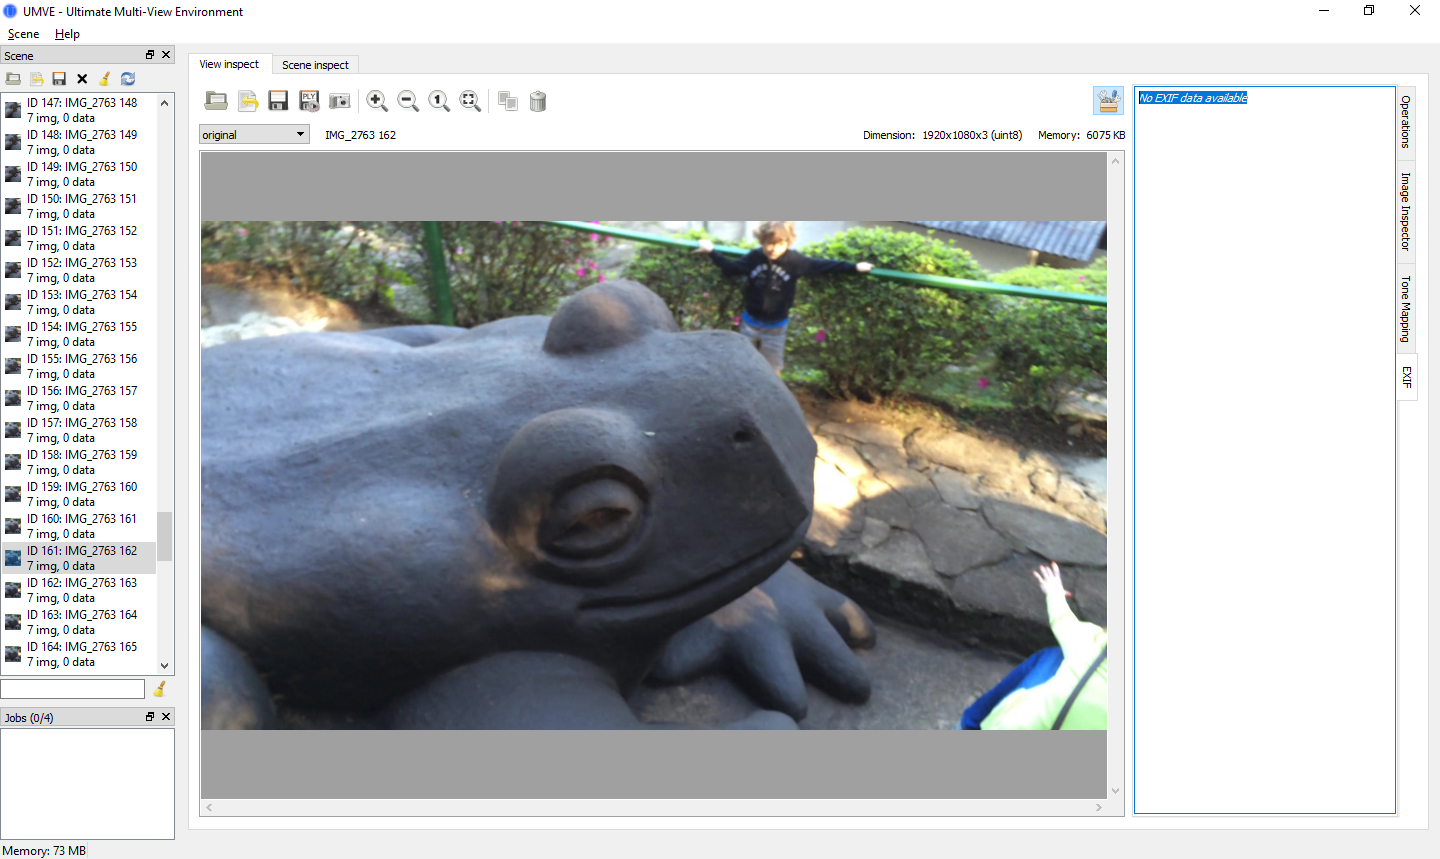
\includegraphics[width=0.5\linewidth]{figs/exifsemumve.png}(b)
	\caption{%
	A figura (a) é um exemplo onde a imagem possui dados na extensão \emph{EXIF} (destacado em azul). Ao passo que a figura (b) é um frame de um vídeo, que não possui os dados das câmeras (destacado em azul).
	%\cite{Cui:Theobalt:etal:PAMI2013,Pajdla:etal:ICCV2011}.
	}\label{fig:mveexif}
\end{figure} 

Foi gerada uma reconstrução de um vídeo gravado de uma escultura no Jardim do Nêgo. O  vídeo foi cortado em \emph{frames} onde foram geradas 200 imagens base, com os parâmetros de câmera gerados pelo próprio software. 

A partir disso, foi executado, todos os passos de uma reconstrução utilizando o MVE, de forma que, foram utilizadas as duas opções, tanto por linha de comando, quanto pela interface gráfica (UMVE).

Pela interface gráfica, o processo todo de reconstrução foi rápido (cerca de 30 minutos) \ref{fig:UMVEdense}, ao passo que por linha de comando, levou cerca de 11 horas e 30 minutos, portanto, vamos nos atentar somente à reconstrução por linha de comando, onde, resumindo, tivemos os resultados~\ref{tab:mveSapo}. 

O UMVE não sinaliza quando o processo em execução termina, então, a explicação para essa discrepância no tempo é devido à execução de outro comando, sobrepondo o que já estava sendo executado, sem que o primeiro tivesse terminado.

\begin{figure}[!h]
	\centering
	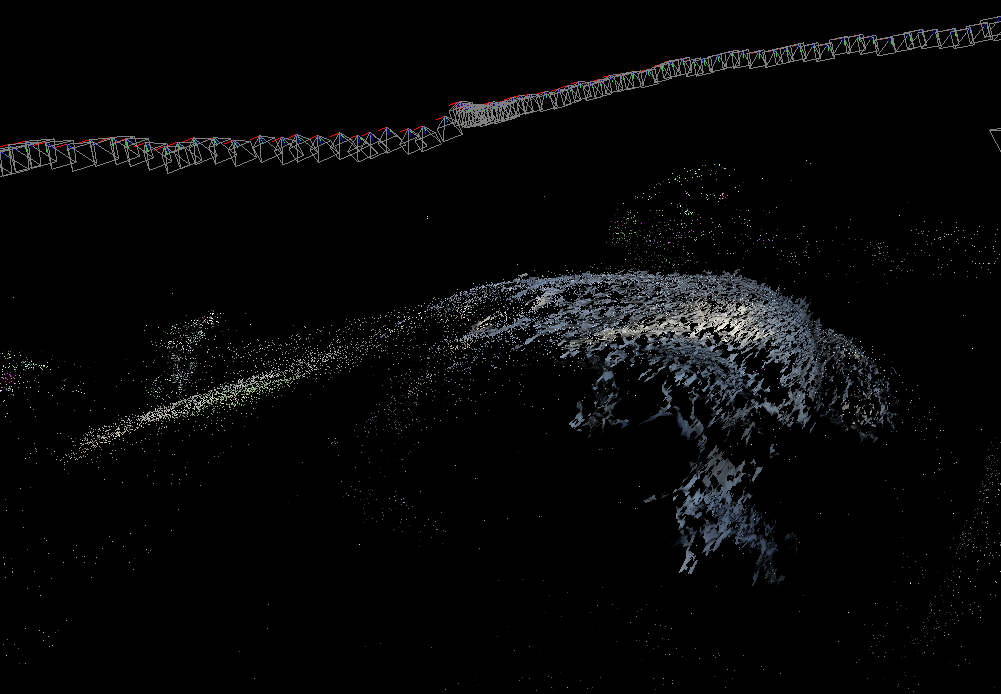
\includegraphics[width=0.5\linewidth]{figs/umvedense.png}
	\caption{%
	Final da reconstrução via UMVE, percebe-se que alguns pontos não foram considerados, tendo como resultado uma "nuvem de pontos" mais densa, basicamente.
	%\cite{Cui:Theobalt:etal:PAMI2013,Pajdla:etal:ICCV2011}.
	}\label{fig:UMVEdense}
\end{figure} 

\begin{table}[!h]
\centering
\caption{Tempos obtidos usando o MVE em um conjunto de dados do Jardim do Nêgo}
\label{tab:mveSapo}
\begin{tabular}{|l|l|}
\hline
Comando            & Tempo (aprox.)    \\ \hline
\emph{sfmrecon}  & 78 segundos     \\ \hline
\emph{dmrecon}   & 14.503 segundos \\ \hline
\emph{scene2pet} & 600 segundos    \\ \hline
\emph{fssrecon}  & 25.293 segundos \\ \hline
\emph{meshclean} & 60 segundos     \\ \hline
\end{tabular}
\end{table}

Na reconstrução por linha de comando também é possível visualizar em qual etapa da execução o algoritmo está (figura~\ref{fig:passosMVE}), configurar alguns parâmetros e inclusive mostrar a porcentagem de progresso do comando em execução. Foram executados os comandos declarados nesta seção.  O \emph{sfmrecon} demorou cerca de 1 minuto e meio \ref{fig:MVESfM}. 

\begin{figure}[!h]
	\centering
	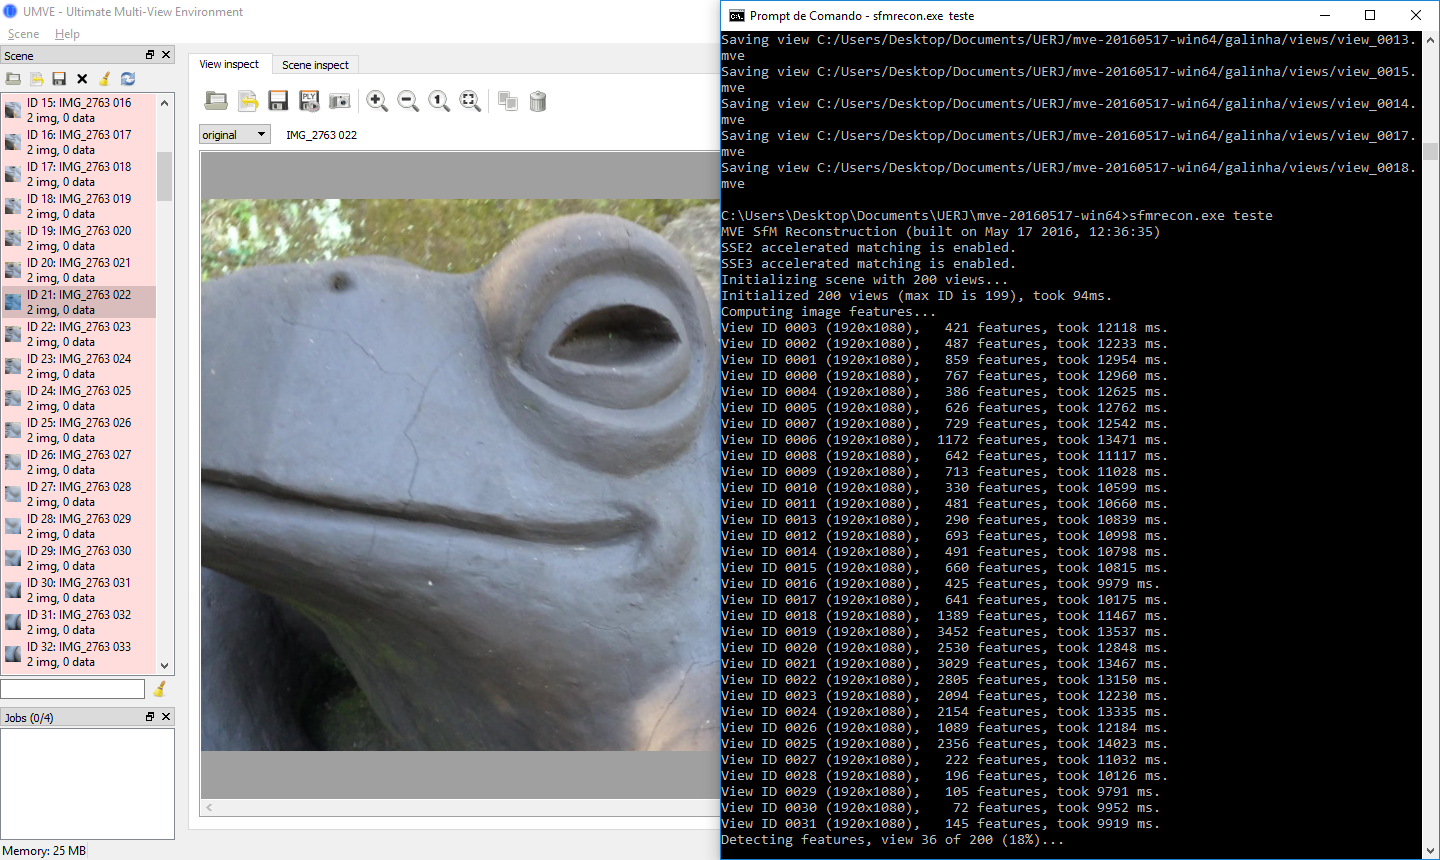
\includegraphics[width=0.45\linewidth]{figs/umve2sfm.png} (a)
	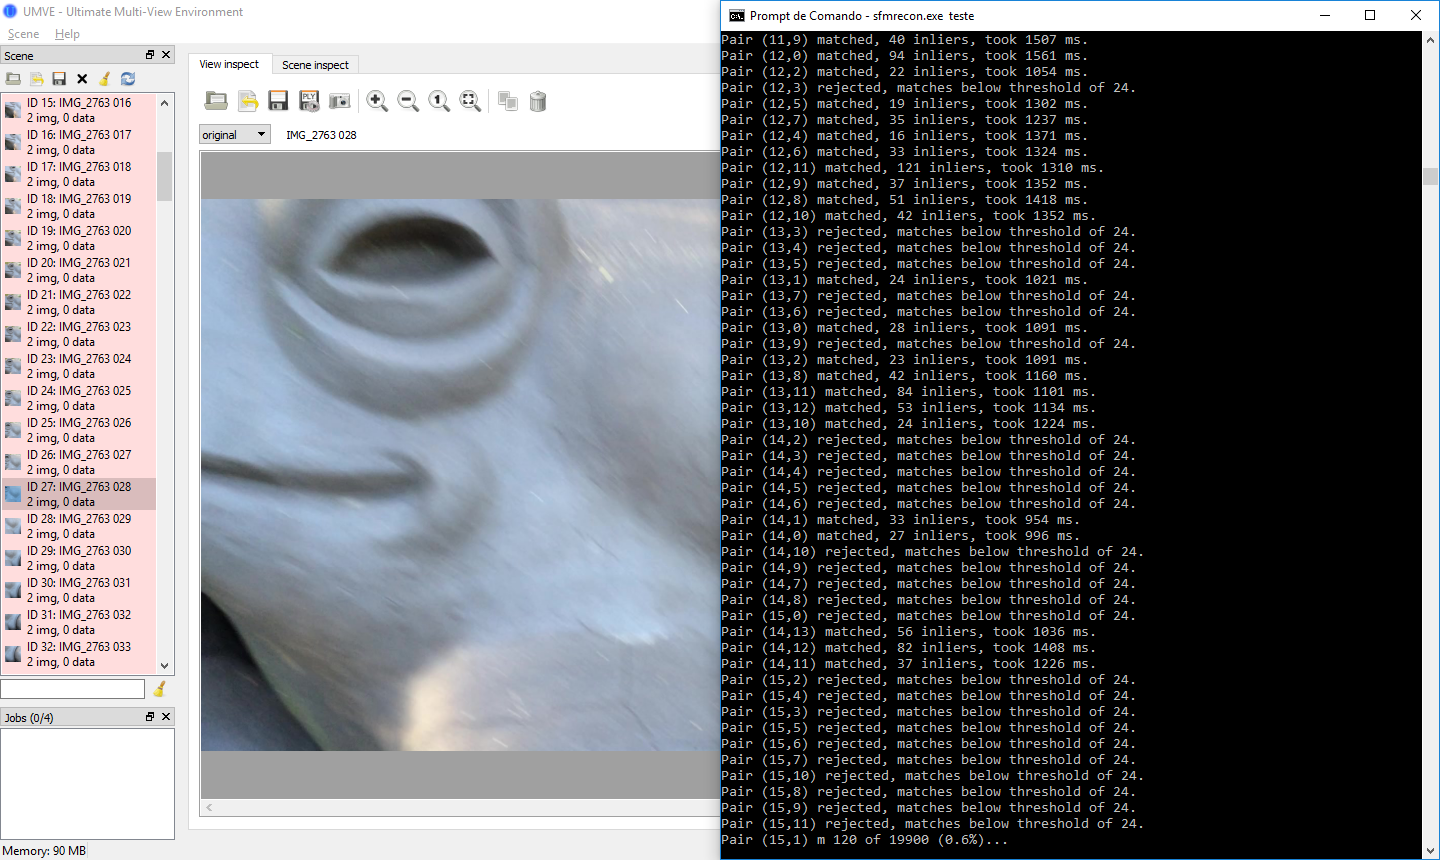
\includegraphics[width=0.45\linewidth]{figs/umve3sfmfeature.png} (b)
	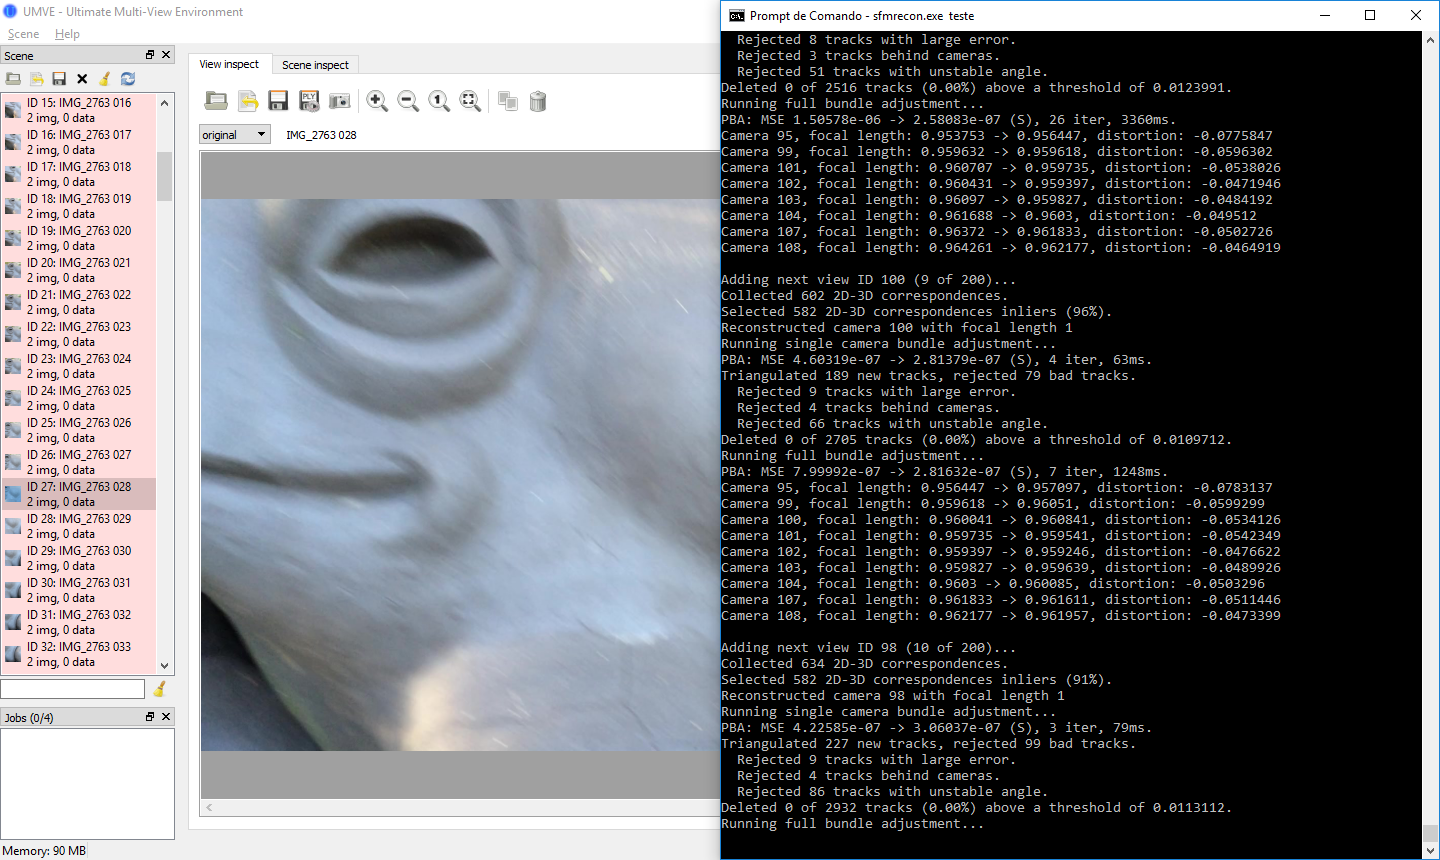
\includegraphics[width=0.45\linewidth]{figs/umve4ba.png} (c)
	\caption{%
	Processos dentro do comando \emph{sfmrecon}, onde (a) estão sendo detectadas as \emph{features} do conjunto de imagens. Em (b) está computado o \emph{pairwise matching} e em (c) está no processo de \emph{Bundle Adjustment}~\cite{bundleAdjustmentSlide}, usando condições-padrão para as câmeras.
	%\cite{Cui:Theobalt:etal:PAMI2013,Pajdla:etal:ICCV2011}.
	}\label{fig:passosMVE}
\end{figure} 

\begin{figure}[h!]
	\centering
	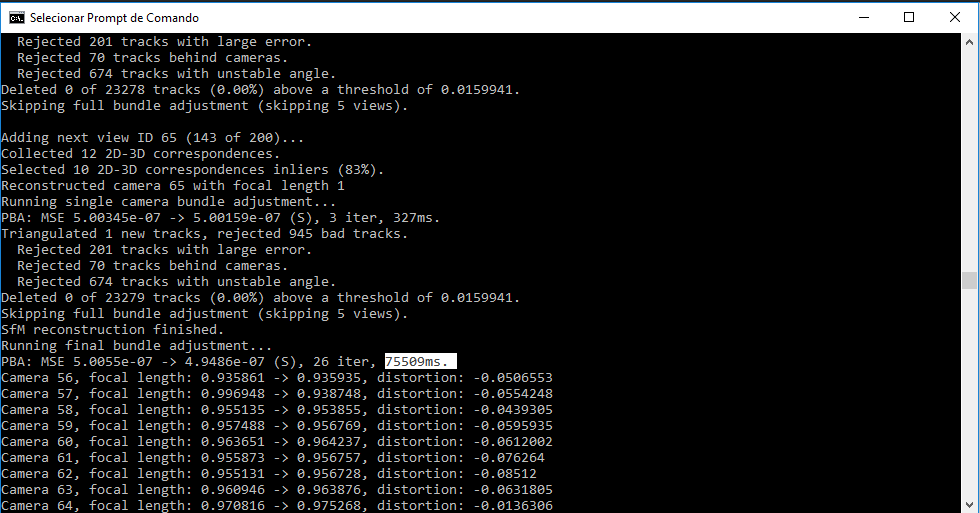
\includegraphics[width=0.65\linewidth]{figs/sfmmve.png}
	\caption{%
	Término do comando \emph{sfmrecon}, onde demorou cerca de 1 minuto e meio (75509 milisegundos).
	%\cite{Cui:Theobalt:etal:PAMI2013,Pajdla:etal:ICCV2011}.
	}\label{fig:MVESfM}
\end{figure}

O próximo comando, \emph{dmrecon} demorou cerca de 4 horas, usando como configuração um nível L2, com 20 vizinhos \ref{fig:MVEDenseRecon}. 
Usando um nível L0, o algoritmo rodou durante 6 horas aproximadamente e foi cancelado devido à demora na execução. 
\newpage %NEWPAGE AQUI%
\begin{figure}[!h]
	\centering
	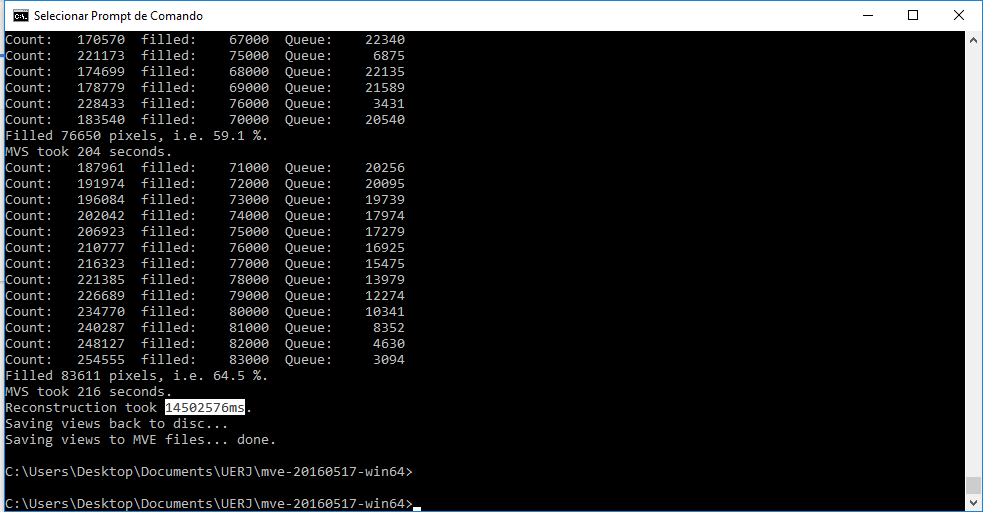
\includegraphics[width=0.8\linewidth]{figs/umvetempo.png}
	\caption{%
	Término do comando \emph{dmrecon}, onde demorou cerca de 4 horas (14502576 milisegundos).
	%\cite{Cui:Theobalt:etal:PAMI2013,Pajdla:etal:ICCV2011}.
	}\label{fig:MVEDenseRecon}
\end{figure} 

Usando o \emph{scene2pet}, é necessário especificarmos em qual nível estamos reconstruindo e também uma saída válida. Por exemplo: "scene2pset.exe -Fnivel cena output". Onde o nível poderá ser um 0 (-F0), 1 (-F1) e assim por diante, a cena é o \emph{input} e o \emph{output} é um arquivo de extensão configurável, neste caso \emph{.ply} \ref{fig:MVEScene2Pet}. Este comando foi rápido, demorou cerca de 10 minutos, levando em conta todos os níveis.

\begin{figure}[!h]
	\centering
	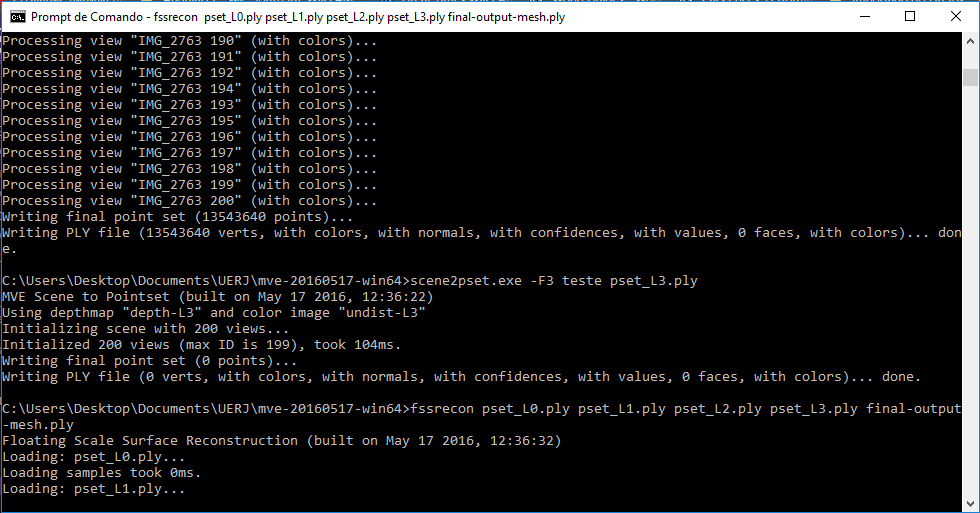
\includegraphics[width=0.8\linewidth]{figs/mvemesh.png}
	\caption{%
	Execução dos comandos \emph{scene2pet}, nos níveis -F0, -F1, -F2 e -F3.
	%\cite{Cui:Theobalt:etal:PAMI2013,Pajdla:etal:ICCV2011}.
	}\label{fig:MVEScene2Pet}
\end{figure} 

Para juntar todos os níveis do \emph{scene2pet}, foi usado o \emph{fssrecon}, que gera uma única reconstrução. Este processo demorou bastante, cerca de 7 horas \ref{fig:MVEFSSR}. Que teve como resultado a malha \ref{fig:MVEFSSRMesh}.
\newpage %NEWPAGE AQUI%

\begin{figure}[!h]
	\centering
	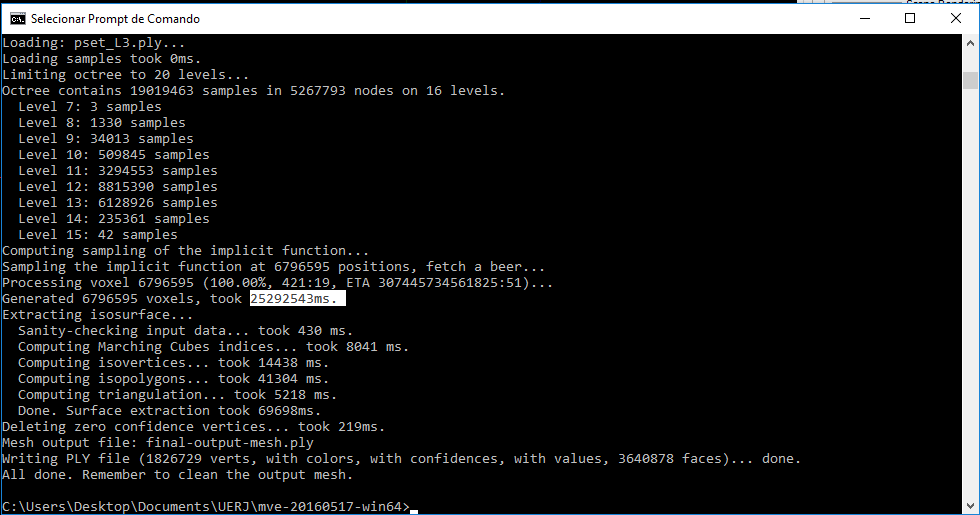
\includegraphics[width=0.8\linewidth]{figs/mvemeshtempo2.png}
	\caption{%
	Progressão do comando \emph{fssrecon}, onde possui o ETA -- \emph{Estimated Time of Arrival}.
	%\cite{Cui:Theobalt:etal:PAMI2013,Pajdla:etal:ICCV2011}.
	}\label{fig:MVEFSSR}
\end{figure} 

\begin{figure}[!h]
	\centering
	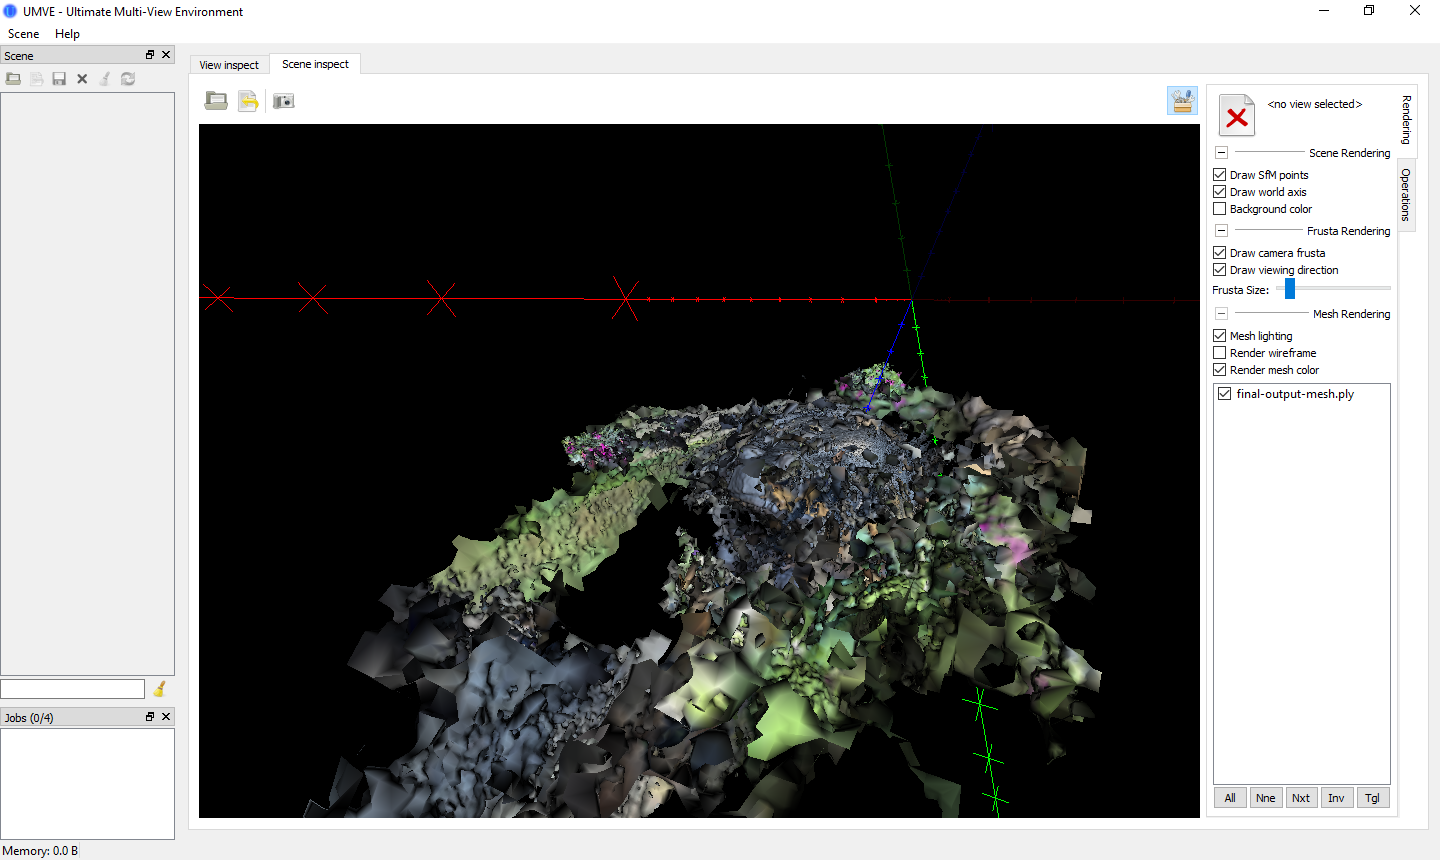
\includegraphics[width=1\linewidth]{figs/mvemeshout.png}
	\caption{%
	Malha com ruídos proveniente do comando \emph{fssrecon}.
	%\cite{Cui:Theobalt:etal:PAMI2013,Pajdla:etal:ICCV2011}.
	}\label{fig:MVEFSSRMesh}
\end{figure} 

Finalmente, basta limpar a malha atual com o comando \emph{meshclean}, onde foi obtido o resultado~\ref{fig:MVEMeshClean}.

\newpage %NEW PAGE AQUI%

\begin{figure}[!h]
	\centering
	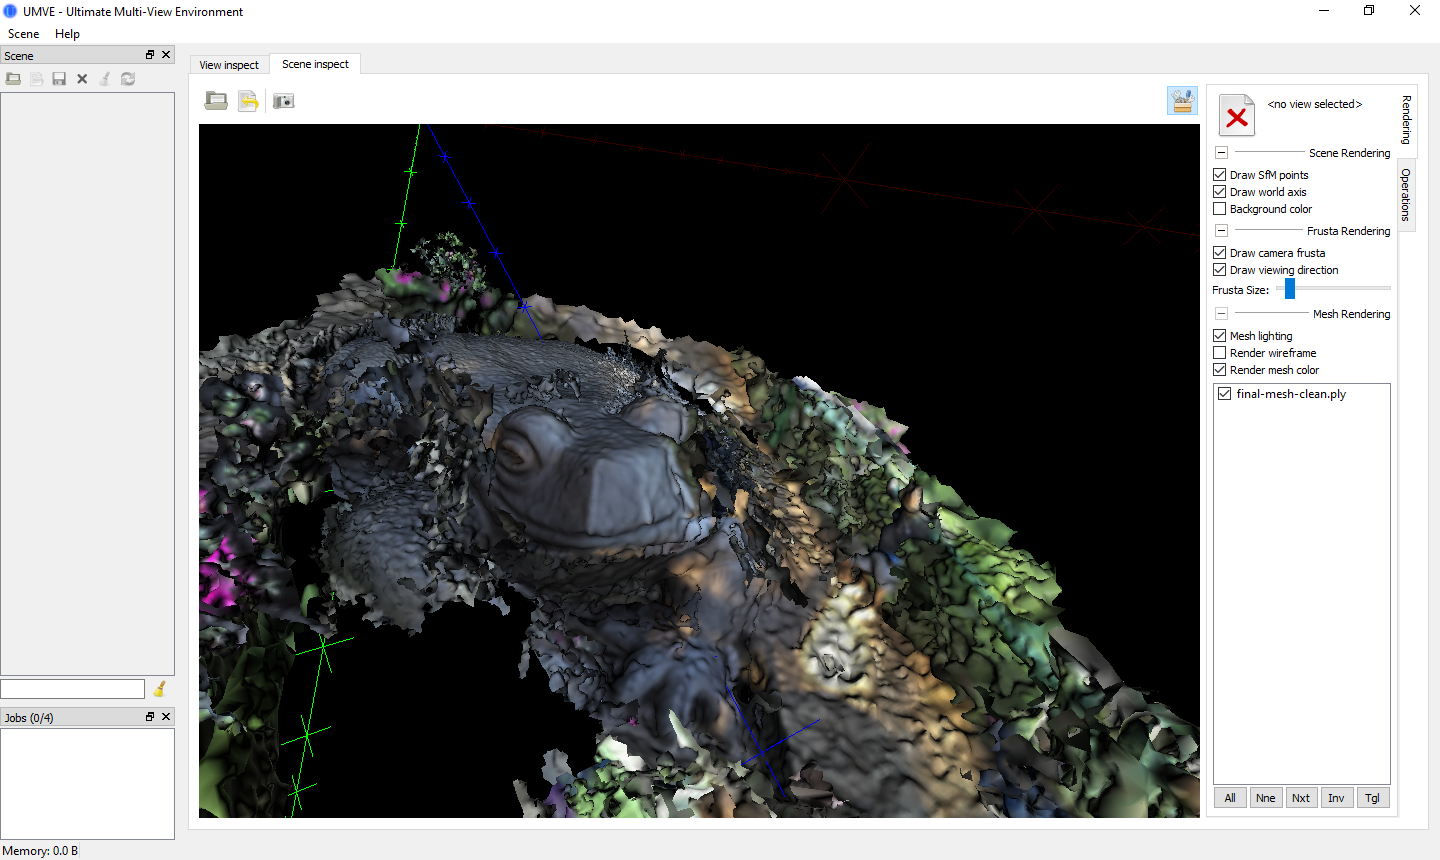
\includegraphics[width=1\linewidth]{figs/mvemeshclean.png}
	\caption{%
	Resultado final, após a remoção dos ruídos da malha.
	%\cite{Cui:Theobalt:etal:PAMI2013,Pajdla:etal:ICCV2011}.
	}\label{fig:MVEMeshClean}
\end{figure} 

Para comparação, usamos o mesmo objeto utilizado na reconstrução do VisualSfM (a galinha) e fizemos o passo a passo com o MVE: com a interface gráfica (UMVE), criamos uma nova cena e inserimos, primeiramente, as 200 fotos do objeto. Em seguida, utilizando as linhas de comando do MVE, fizemos o procedimento padrão de reconstrução do software. E, obtivemos os seguintes resultados~\ref{tab:galinha200mve}:

\begin{table}[!h]
\centering
\caption{Tempos obtidos usando o MVE em um conjunto de dados em ambiente interno com 200 imagens}
\label{tab:galinha200mve}
\begin{tabular}{|l|l|}
\hline
Comando            & Tempo (aprox.)         \\ \hline
\emph{sfmrecon}  & 371 segundos   \\ \hline
\emph{dmrecon}   & 3.716 segundos \\ \hline
\emph{scene2pet} & 300 segundos   \\ \hline
\emph{fssrecon}  & 1.695 segundos \\ \hline
\emph{meshclean} & 45 segundos    \\ \hline
\end{tabular}
\end{table}

\begin{figure}[!h]
	\centering
	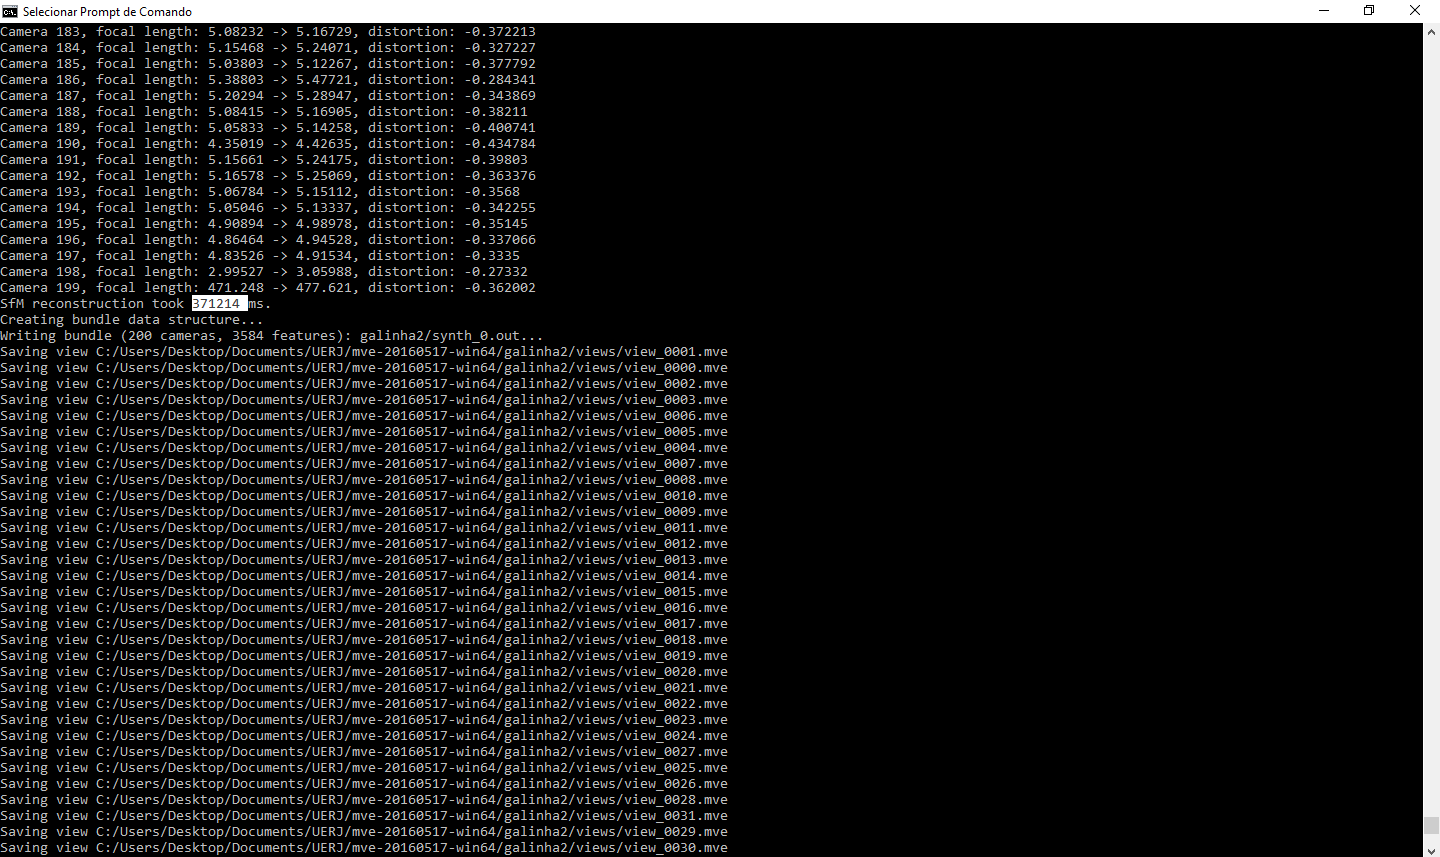
\includegraphics[width=0.5\linewidth]{figs/galinhalongesfmreconmve.png}
	\caption{%
	Tempo gasto da etapa \emph{sfmrecon} do MVE
	}\label{fig:sfmrecon1}
\end{figure}

\begin{figure}[!h]
	\centering
	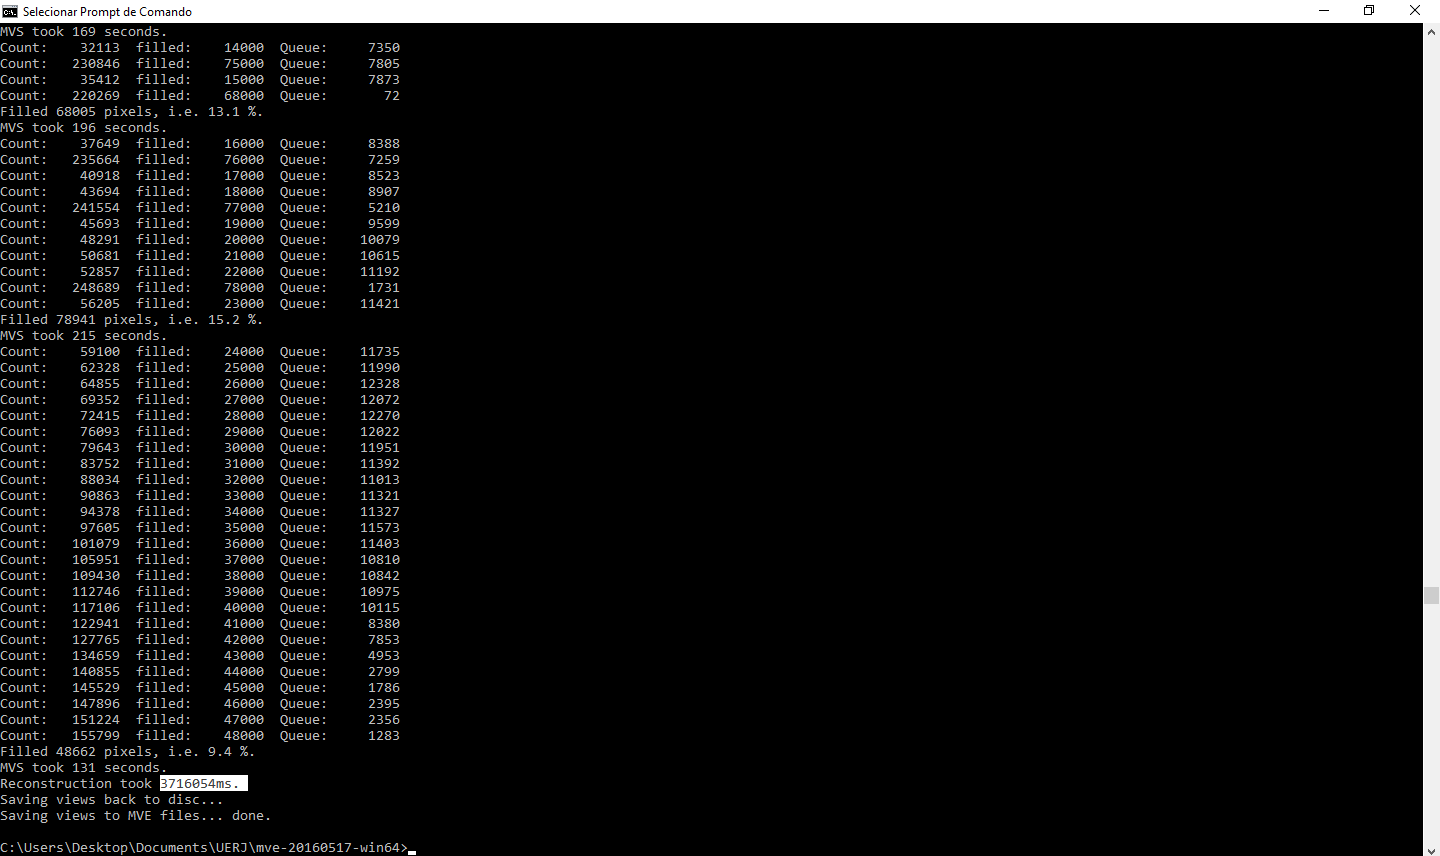
\includegraphics[width=0.5\linewidth]{figs/galinhadmreconmve.png}
	\caption{%
	Tempo da etapa \emph{dmrecon} do MVE
	%\cite{Cui:Theobalt:etal:PAMI2013,Pajdla:etal:ICCV2011}.
	}\label{fig:dmrecon1}
\end{figure}

\begin{figure}[!h]
	\centering
	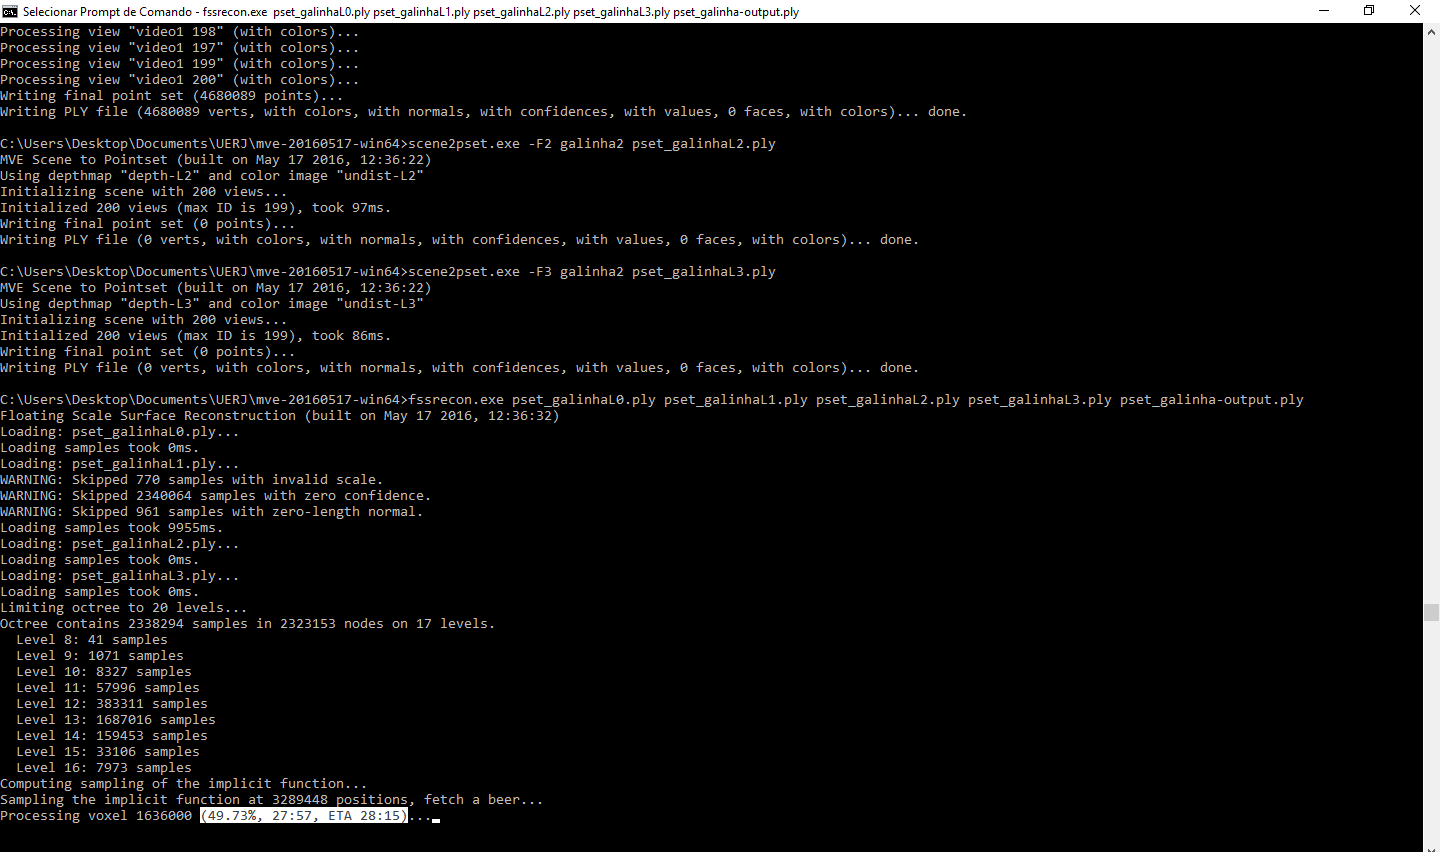
\includegraphics[width=0.5\linewidth]{figs/mvefssrecongalinha.png}
	\caption{%
	Tempo da etapa \emph{fssrecon} do MVE
	%\cite{Cui:Theobalt:etal:PAMI2013,Pajdla:etal:ICCV2011}.
	}\label{fig:fssrecon}
\end{figure}

\begin{figure}[!h]
	\centering
	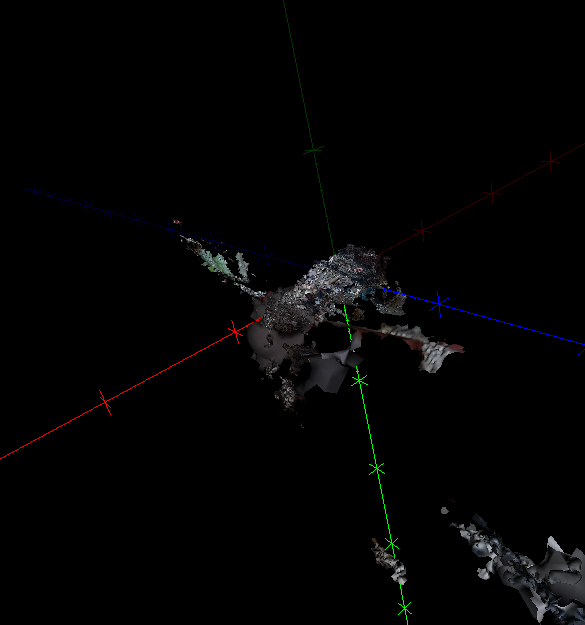
\includegraphics[width=0.5\linewidth]{figs/galinhadmr.png}
	\caption{%
	Resultado da etapa \emph{fssrecon} do MVE
	%\cite{Cui:Theobalt:etal:PAMI2013,Pajdla:etal:ICCV2011}.
	}\label{fig:galinhaFssr}
\end{figure}

\begin{figure}[!h]
	\centering
	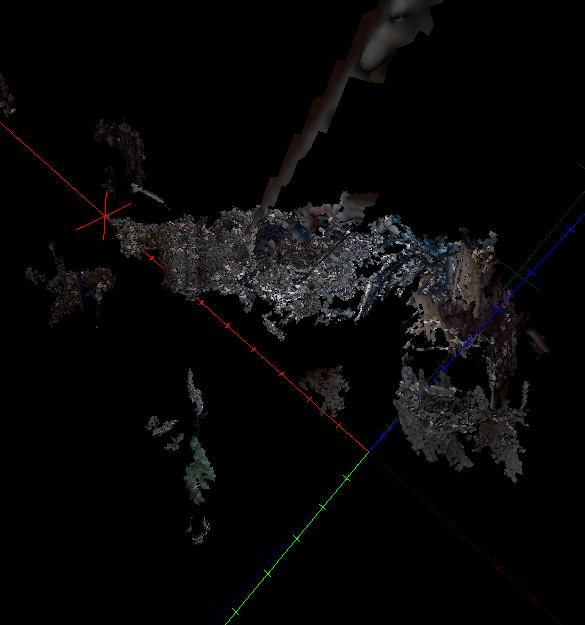
\includegraphics[width=0.5\linewidth]{figs/galinhameshclean.png}
	\caption{%
	Resultado da etapa \emph{meshclean}, da etapa anterior \ref{fig:galinhaFssr}
	%\cite{Cui:Theobalt:etal:PAMI2013,Pajdla:etal:ICCV2011}.
	}\label{fig:galinhaMeshClean}
\end{figure}

A etapa de \emph{scene2pset} demorou cerca de 20 segundos (total). Porém percebemos que a reconstrução não foi satisfatória, o \emph{software} se confundiu, e não conseguiu obter os parâmetros corretos das câmeras utilizadas. A partir disso, o erro se propagou e gerou essa reconstrução acima \ref{fig:galinhaFssr} e \ref{fig:galinhaMeshClean}.

Rodamos também, com as 224 fotos, só foi possível executar o passo \emph{sfmrecon} \ref{fig:galinhaSfM224}, pois o MVE não conseguiu rodar o comando \emph{dmrecon} por algum motivo, e não gerou nenhum resultado para a continuação do algoritmo \ref{fig:galinhaDMR224}.

\begin{figure}[!h]
	\centering
	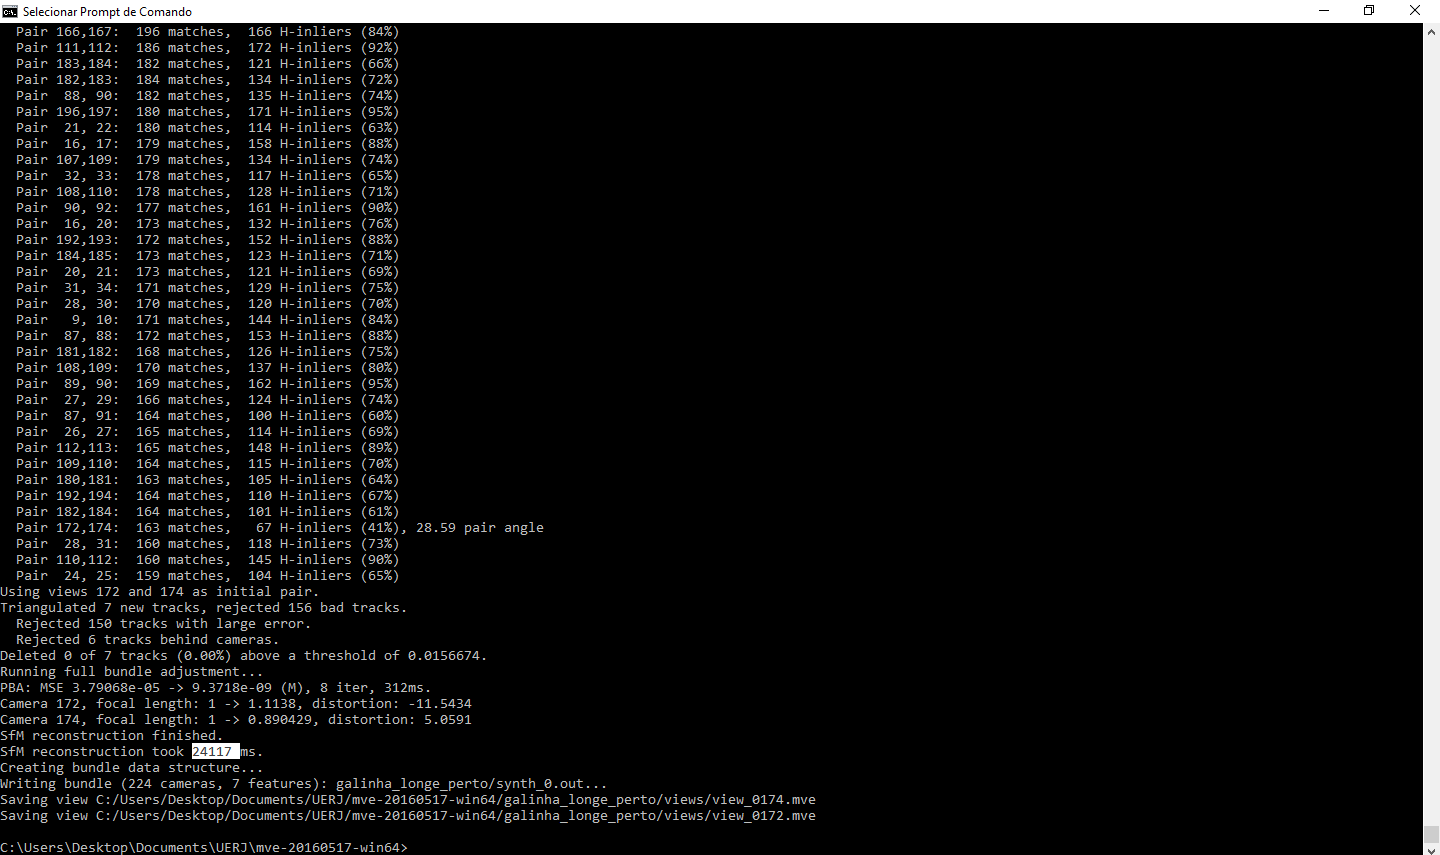
\includegraphics[width=0.5\linewidth]{figs/mvesfmrecongalinhapertolonge.png}
	\caption{%
	Resultado da etapa \emph{sfmrecon}, com todas as imagens
	%\cite{Cui:Theobalt:etal:PAMI2013,Pajdla:etal:ICCV2011}.
	}\label{fig:galinhaSfM224}
\end{figure}

\begin{figure}[!h]
	\centering
	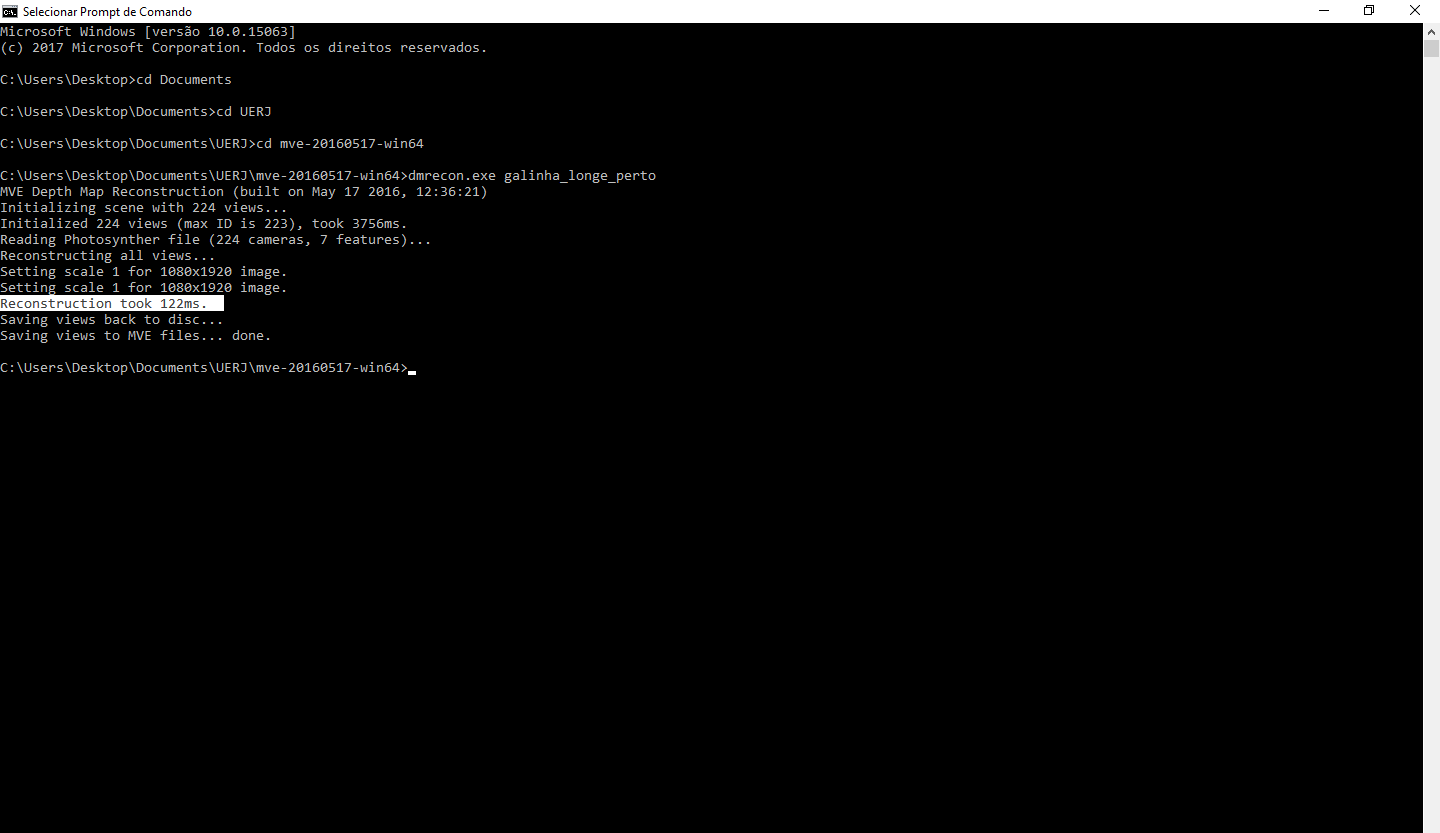
\includegraphics[width=0.5\linewidth]{figs/mvedmrecongalinhapertolonge.png}
	\caption{%
	Resultado da etapa \emph{dmrecon}, com todas as imagens
	%\cite{Cui:Theobalt:etal:PAMI2013,Pajdla:etal:ICCV2011}.
	}\label{fig:galinhaDMR224}
\end{figure}

